% Generated by ops/build_paper_inference_followups.py; do not edit numbers.
\section{Inference: Adaptation, Model Mixtures, and Coarser Keys}
\label{app:inference-followups}
We evaluate adaptation to changed requirements, complementarity between
models, and sensitivity to the definition of a solution mode. Model weights
remain fixed during inference. Pointwise 95\% percentile intervals use 20,000
paired whole-problem bootstrap replicates. Resampling preserves all
perturbations, model conditions, and training seeds for each problem;
hosted comparisons resample within each domain and level. These intervals
condition on the observed response pools and training seeds, so they do not
estimate variability across new response pools or training seeds. The 21
model-pair comparisons are dependent, and intervals are unadjusted for
multiple comparisons.

\subsection{\texttt{PantryPlan} portfolios under changed requirements}
\label{app:pantry-adaptation}
We evaluate the initial Qwen2.5-0.5B checkpoint and Level-2 Dr.GRPO and
Re:Dr checkpoints from two matched training seeds on 32 held-out problems.
We derive 192 single-ingredient outages from the task specifications,
independently of generated answers. Exhaustive search over the original
quantity grid finds valid plans for 181 revised tasks. These plans establish
feasibility and are withheld from the model. Five feasible additional dietary
restrictions are reported separately, as they cover only five source problems.

Each portfolio contains eight plans, which we test unchanged against the
revised requirements. If none remains valid, we allow up to eight sequential
recovery calls and stop at the first valid plan. Unresolved portfolios use
all eight calls. Each recovery prompt contains the revised task, initial
portfolio, previous recovery outputs, and deterministic verifier feedback.
Cumulative success includes portfolios that require no recovery. We average
over perturbations within each source problem, then weight problems equally.

The three sampling strategies use the same checkpoints, verifier, and
192-token response cap. Ordinary sampling uses temperature 1.0. Temperature
tuning selects from $\{0.7,1.0,1.3\}$ based on outage survival on 16 separate
development problems (384 responses per checkpoint). Diversity prompting
makes eight sequential calls, requesting a plan with a new ingredient support
and retaining the complete output history, including failures. All strategies
use the same number of initial responses, but their context lengths and total
token costs differ.

\begin{figure}[!htbp]
\centering
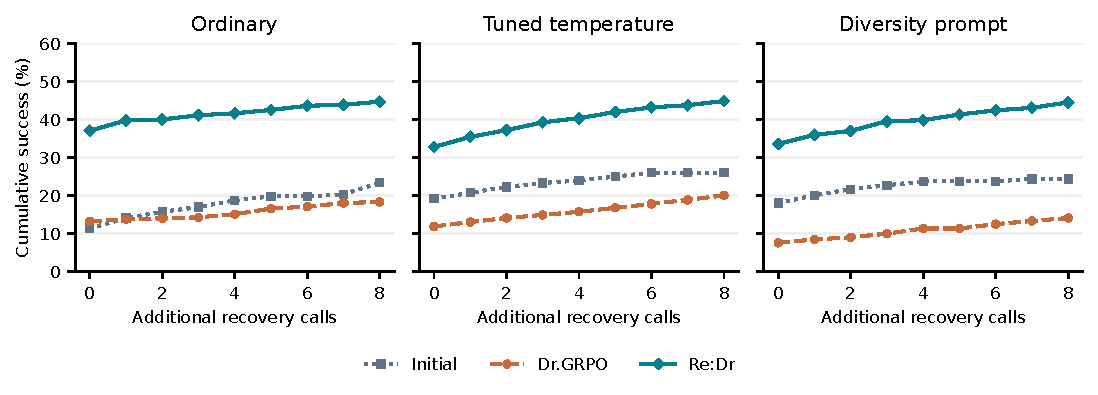
\includegraphics[width=\linewidth]{figures/pantry_adaptation_recovery_20260912.pdf}
\caption{\textbf{Re:Dr improves portfolio survival and success within eight
recovery calls.} Panels compare ordinary sampling, tuned temperature, and
diversity prompting on the same 181 feasible ingredient outages from 32
\texttt{PantryPlan} problems. The horizontal axis is the additional recovery-call budget;
the vertical axis includes success without recovery at zero calls. Curves
average outages within problems, then problems equally. Solid diamonds show
Re:Dr, dashed circles Dr.GRPO, and dotted squares the initial checkpoint;
trained curves average two matched seeds. Pointwise 95\% intervals for
paired differences appear in Table~\ref{tab:pantry-adaptation-contrasts}.}
\label{fig:pantry-adaptation-recovery}
\end{figure}

\begin{table}[!htbp]
\centering
\caption{\textbf{Re:Dr portfolios adapt better to ingredient outages across all three sampling strategies.} Eight initial plans face 181 feasible outages from 32 problems or five additional dietary restrictions from five problems. Survival is success without recovery; By 8 includes success within eight recovery calls (both percentages). Calls count unresolved cases as eight. Token totals count the initial portfolio once per revised task. Entries average perturbations within problems, then problems equally; dietary estimates use only five problems. Labels (a) and (b) denote the two matched training replicates.}
\label{tab:pantry-adaptation}
\scriptsize
\setlength{\tabcolsep}{3pt}
\begin{tabular}{lllrrrrr}
\toprule
Change & Checkpoint & Strategy & Survival & By 8 & Calls & Input tokens & Output tokens \\
\midrule
Outages & Initial & Ordinary & 11.35 & 23.44 & 6.63 & 11301.75 & 376.49 \\
 & Initial & Tuned temperature & 19.17 & 26.04 & 6.13 & 10864.88 & 370.17 \\
 & Initial & Diversity prompt & 18.02 & 24.38 & 6.22 & 11794.81 & 352.87 \\
 & Dr.GRPO (a) & Ordinary & 9.79 & 14.01 & 7.09 & 12439.22 & 823.70 \\
 & Dr.GRPO (a) & Tuned temperature & 13.44 & 16.77 & 6.79 & 12017.57 & 775.44 \\
 & Dr.GRPO (a) & Diversity prompt & 5.21 & 8.39 & 7.44 & 14103.23 & 848.09 \\
 & Dr.GRPO (b) & Ordinary & 16.67 & 22.60 & 6.47 & 11265.39 & 637.59 \\
 & Dr.GRPO (b) & Tuned temperature & 10.31 & 23.39 & 6.75 & 11531.40 & 644.94 \\
 & Dr.GRPO (b) & Diversity prompt & 9.90 & 19.79 & 6.90 & 13124.10 & 731.00 \\
 & Re:Dr (a) & Ordinary & 39.38 & 47.97 & 4.47 & 9078.92 & 297.98 \\
 & Re:Dr (a) & Tuned temperature & 28.23 & 40.94 & 5.19 & 9718.01 & 310.50 \\
 & Re:Dr (a) & Diversity prompt & 36.93 & 47.19 & 4.68 & 10465.22 & 344.02 \\
 & Re:Dr (b) & Ordinary & 34.74 & 41.51 & 4.94 & 9547.16 & 308.52 \\
 & Re:Dr (b) & Tuned temperature & 37.34 & 48.85 & 4.53 & 9148.77 & 300.05 \\
 & Re:Dr (b) & Diversity prompt & 30.26 & 41.93 & 5.06 & 10584.02 & 313.50 \\
\midrule
Dietary & Initial & Ordinary & 0.00 & 20.00 & 6.80 & 11392.80 & 371.20 \\
 & Initial & Tuned temperature & 20.00 & 40.00 & 6.40 & 11175.20 & 387.20 \\
 & Initial & Diversity prompt & 0.00 & 0.00 & 8.00 & 13630.20 & 405.00 \\
 & Dr.GRPO (a) & Ordinary & 0.00 & 0.00 & 8.00 & 13310.20 & 849.20 \\
 & Dr.GRPO (a) & Tuned temperature & 0.00 & 0.00 & 8.00 & 13394.60 & 856.00 \\
 & Dr.GRPO (a) & Diversity prompt & 0.00 & 0.00 & 8.00 & 15045.40 & 939.60 \\
 & Dr.GRPO (b) & Ordinary & 0.00 & 20.00 & 7.40 & 12063.00 & 650.40 \\
 & Dr.GRPO (b) & Tuned temperature & 0.00 & 0.00 & 8.00 & 12544.20 & 615.40 \\
 & Dr.GRPO (b) & Diversity prompt & 0.00 & 0.00 & 8.00 & 14132.40 & 725.60 \\
 & Re:Dr (a) & Ordinary & 20.00 & 60.00 & 5.20 & 9732.60 & 326.00 \\
 & Re:Dr (a) & Tuned temperature & 40.00 & 40.00 & 4.80 & 9402.80 & 307.60 \\
 & Re:Dr (a) & Diversity prompt & 40.00 & 40.00 & 4.80 & 10693.60 & 355.60 \\
 & Re:Dr (b) & Ordinary & 40.00 & 80.00 & 3.20 & 7853.20 & 271.20 \\
 & Re:Dr (b) & Tuned temperature & 40.00 & 80.00 & 3.60 & 8127.80 & 265.20 \\
 & Re:Dr (b) & Diversity prompt & 20.00 & 40.00 & 5.00 & 10738.20 & 341.00 \\
\bottomrule
\end{tabular}
\end{table}


\begin{table}[!htbp]
\centering
\caption{\textbf{Re:Dr raises outage survival and reduces recovery calls.} Entries are Re:Dr minus Dr.GRPO, averaged over two matched seeds on 32 paired problems. Survival and success by eight calls are percentage-point differences; calls include unresolved cases. Brackets are pointwise 95\% paired problem-bootstrap intervals, conditional on the observed training seeds.}
\label{tab:pantry-adaptation-contrasts}
\scriptsize
\setlength{\tabcolsep}{3pt}
\begin{tabular}{lrrr}
\toprule
Strategy & $\Delta$ survival & $\Delta$ by 8 calls & $\Delta$ calls \\
\midrule
Ordinary & $23.83$ $[12.16, 35.89]$ & $26.43$ $[14.69, 38.18]$ & $-2.08$ $[-3.03, -1.14]$ \\
Tuned temperature & $20.91$ $[9.19, 32.89]$ & $24.82$ $[14.04, 35.52]$ & $-1.91$ $[-2.78, -1.05]$ \\
Diversity prompt & $26.04$ $[16.93, 35.65]$ & $30.47$ $[21.51, 39.27]$ & $-2.30$ $[-3.04, -1.57]$ \\
\bottomrule
\end{tabular}
\end{table}

With ordinary sampling, Re:Dr improves survival over Dr.GRPO by 23.83 percentage points
$[12.16,35.89]$, reduces the mean number of recovery calls, capped at eight, by 2.08
$[1.14,3.03]$, and improves success within eight recovery calls by 26.43 points
$[14.69,38.18]$. Mean input and output token totals fall by 2,539.27
$[1,618.01,3,468.86]$ and 427.40 $[386.83,466.30]$, respectively.
The initial portfolios also contain 1.234 more correct responses out of
eight $[.578,1.984]$. Restricting each paired-seed comparison to portfolios
with equal observed correct counts leaves a 1.05-percentage-point survival
gain $[0.00,3.53]$. We first average eligible seed comparisons within each
problem, then average the 19 problems with at least one eligible comparison.
This restriction changes both the problem and seed composition, and equal
observed counts do not establish equal underlying accuracy. The adaptation
gains therefore do not isolate diversity as their causal mechanism.

Per-perturbation token totals represent deploying one portfolio and recovering
from one change in requirements. Input counts include reused prefixes and
do not measure the compute saved by prefix caching. Table~\ref{tab:pantry-collection-cost}
counts each response once across temperature selection, initial portfolios
from tuned-temperature sampling and diversity prompting, and recovery under
all three strategies. It excludes ordinary initial-portfolio generation.
Neither inference cost summary includes training costs.

\begin{table}[!htbp]
\centering
\caption{\textbf{Inference costs include temperature selection and recovery.} Each checkpoint selects $T$ from 384 responses on 16 development problems. Inference totals include this calibration, initial portfolios for tuned-temperature and diversity prompting, and recovery under all three strategies on 32 evaluation problems. Ordinary initial-portfolio generation is excluded. Each response is counted once, including reused input prefixes. Seconds report generation time, excluding training, without hardware normalization. Labels (a) and (b) denote matched training replicates.}
\label{tab:pantry-collection-cost}
\scriptsize
\setlength{\tabcolsep}{3pt}
\begin{tabular}{llrrrrr}
\toprule
Checkpoint & Scope & $T$ & Responses & Input tokens & Output tokens & Seconds \\
\midrule
Dr.GRPO (a) & Calibration & 1.3 & 384 & 229392 & 19871 & 136.3 \\
Dr.GRPO (a) & Inference total & 1.3 & 4874 & 4870884 & 272484 & 3302.0 \\
Dr.GRPO (b) & Calibration & 1.3 & 384 & 229392 & 15544 & 126.5 \\
Dr.GRPO (b) & Inference total & 1.3 & 4634 & 4365524 & 220458 & 2792.9 \\
Re:Dr (a) & Calibration & 0.7 & 384 & 229392 & 8552 & 111.1 \\
Re:Dr (a) & Inference total & 0.7 & 3559 & 3160284 & 92227 & 1527.7 \\
Re:Dr (b) & Calibration & 1.0 & 384 & 229392 & 8585 & 112.5 \\
Re:Dr (b) & Inference total & 1.0 & 3592 & 3169337 & 88300 & 1510.2 \\
Initial & Calibration & 1.3 & 384 & 229392 & 9521 & 123.5 \\
Initial & Inference total & 1.3 & 4416 & 4035069 & 116619 & 1957.4 \\
\bottomrule
\end{tabular}
\end{table}


\subsection{Complementarity across hosted models}
\label{app:cross-model-overlap}
Seven hosted models each produce eight responses to the same 1,920 prompts
(five domains, three levels, and 128 prompts per domain and level), totaling
107,520 responses. We use strict grading and the original Opus 5 \texttt{Python}
interface; the formatting-normalized hosted comparison uses a revised
Opus 5 interface. For each of the 21 model pairs, a mixed portfolio draws four
responses without replacement from each model's eight-response pool. We
compute its expected distinct-mode count exactly over all $\binom{8}{4}^2=4{,}900$
subset pairs, then compare with each constituent's complete eight-response
portfolio and their average. These are expectations within the finite
response pools, conditional on the outputs generated.

Every mixture increases the expected number of distinct solution modes
relative to its average constituent by $.115$--$.266$. Ten pairs improve
on both constituents in point estimates; nine have pointwise intervals
entirely above zero against both. On
prompts with at least four correct responses from each model, we also compare
a mixture of two correct draws per model with four correct draws from either
constituent. All pairwise gains over the average constituent remain positive
($.073$--$.177$ modes). Fixing the number of correct draws conditions on a
different eligible subset for each pair. It does not equate accuracy or the
number of attempts required to obtain those correct responses.

\begin{table}[!htbp]
\centering
\caption{\textbf{Every model pair increases expected distinct modes over its average constituent.} A 4+4 mixture samples without replacement from the two eight-response pools; A and B name the constituents in order. Panel A compares with their average: fine and coarse keys use all 1,920 prompts, while the four-correct-draw comparison uses $n$ prompts with at least four correct responses per model (2+2 mixed versus four per constituent). Panel B compares fine-key distinct modes with each constituent and pass@8 with their average. Entries are distinct-mode differences except pass@8, in percentage points. Brackets are pointwise 95\% paired problem-bootstrap intervals, stratified by domain and level; comparisons share models and prompts.}
\label{tab:cross-model-mixtures}
\scriptsize
\setlength{\tabcolsep}{3pt}
\textbf{A}\par\smallskip
\resizebox{\linewidth}{!}{%
\begin{tabular}{lrrrr}
\toprule
Pair & Fine & Coarse & Four correct draws & $n$ \\
\midrule
DeepSeek V4 Pro + Kimi K3 & $0.148$ $[0.136, 0.160]$ & $0.142$ $[0.131, 0.154]$ & $0.107$ $[0.098, 0.115]$ & 1858 \\
DeepSeek V4 Pro + Opus 4.8 & $0.198$ $[0.185, 0.211]$ & $0.183$ $[0.171, 0.197]$ & $0.153$ $[0.142, 0.164]$ & 1847 \\
DeepSeek V4 Pro + Opus 5 & $0.262$ $[0.249, 0.275]$ & $0.252$ $[0.240, 0.265]$ & $0.177$ $[0.165, 0.190]$ & 1510 \\
DeepSeek V4 Pro + GPT-5.4 & $0.133$ $[0.122, 0.143]$ & $0.127$ $[0.116, 0.138]$ & $0.098$ $[0.090, 0.107]$ & 1695 \\
DeepSeek V4 Pro + GPT-5.6 Sol & $0.235$ $[0.223, 0.247]$ & $0.224$ $[0.212, 0.237]$ & $0.154$ $[0.142, 0.166]$ & 1396 \\
DeepSeek V4 Pro + Grok 4.3 & $0.123$ $[0.112, 0.134]$ & $0.117$ $[0.106, 0.127]$ & $0.091$ $[0.083, 0.099]$ & 1859 \\
Kimi K3 + Opus 4.8 & $0.187$ $[0.174, 0.200]$ & $0.172$ $[0.159, 0.185]$ & $0.138$ $[0.127, 0.148]$ & 1885 \\
Kimi K3 + Opus 5 & $0.266$ $[0.253, 0.279]$ & $0.255$ $[0.242, 0.268]$ & $0.162$ $[0.150, 0.175]$ & 1543 \\
Kimi K3 + GPT-5.4 & $0.127$ $[0.115, 0.139]$ & $0.112$ $[0.101, 0.124]$ & $0.083$ $[0.075, 0.092]$ & 1720 \\
Kimi K3 + GPT-5.6 Sol & $0.202$ $[0.190, 0.214]$ & $0.195$ $[0.183, 0.207]$ & $0.093$ $[0.083, 0.104]$ & 1417 \\
Kimi K3 + Grok 4.3 & $0.115$ $[0.104, 0.126]$ & $0.110$ $[0.099, 0.121]$ & $0.073$ $[0.066, 0.080]$ & 1900 \\
Opus 4.8 + Opus 5 & $0.187$ $[0.176, 0.199]$ & $0.182$ $[0.171, 0.193]$ & $0.098$ $[0.087, 0.109]$ & 1534 \\
Opus 4.8 + GPT-5.4 & $0.201$ $[0.186, 0.215]$ & $0.185$ $[0.172, 0.199]$ & $0.156$ $[0.144, 0.168]$ & 1713 \\
Opus 4.8 + GPT-5.6 Sol & $0.247$ $[0.234, 0.261]$ & $0.237$ $[0.223, 0.250]$ & $0.151$ $[0.138, 0.164]$ & 1409 \\
Opus 4.8 + Grok 4.3 & $0.180$ $[0.167, 0.194]$ & $0.171$ $[0.158, 0.184]$ & $0.141$ $[0.130, 0.153]$ & 1894 \\
Opus 5 + GPT-5.4 & $0.228$ $[0.215, 0.241]$ & $0.217$ $[0.204, 0.230]$ & $0.158$ $[0.145, 0.171]$ & 1493 \\
Opus 5 + GPT-5.6 Sol & $0.169$ $[0.157, 0.182]$ & $0.161$ $[0.149, 0.174]$ & $0.143$ $[0.130, 0.156]$ & 1370 \\
Opus 5 + Grok 4.3 & $0.231$ $[0.219, 0.244]$ & $0.225$ $[0.213, 0.237]$ & $0.145$ $[0.133, 0.157]$ & 1547 \\
GPT-5.4 + GPT-5.6 Sol & $0.156$ $[0.145, 0.167]$ & $0.147$ $[0.136, 0.158]$ & $0.094$ $[0.084, 0.104]$ & 1400 \\
GPT-5.4 + Grok 4.3 & $0.130$ $[0.119, 0.142]$ & $0.121$ $[0.111, 0.132]$ & $0.095$ $[0.086, 0.104]$ & 1722 \\
GPT-5.6 Sol + Grok 4.3 & $0.211$ $[0.199, 0.224]$ & $0.204$ $[0.192, 0.216]$ & $0.118$ $[0.107, 0.130]$ & 1418 \\
\bottomrule
\end{tabular}
}
\par\medskip
\textbf{B}\par\smallskip
\resizebox{\linewidth}{!}{%
\begin{tabular}{lrrr}
\toprule
Pair & $\Delta D$ vs A & $\Delta D$ vs B & $\Delta$ pass@8 vs mean \\
\midrule
DeepSeek V4 Pro + Kimi K3 & $0.279$ $[0.254, 0.304]$ & $0.017$ $[-0.008, 0.043]$ & $0.22$ $[0.08, 0.39]$ \\
DeepSeek V4 Pro + Opus 4.8 & $0.089$ $[0.064, 0.114]$ & $0.307$ $[0.282, 0.332]$ & $0.31$ $[0.15, 0.49]$ \\
DeepSeek V4 Pro + Opus 5 & $-0.061$ $[-0.082, -0.039]$ & $0.585$ $[0.560, 0.610]$ & $7.48$ $[7.19, 7.78]$ \\
DeepSeek V4 Pro + GPT-5.4 & $0.097$ $[0.074, 0.121]$ & $0.168$ $[0.145, 0.192]$ & $0.64$ $[0.41, 0.90]$ \\
DeepSeek V4 Pro + GPT-5.6 Sol & $-0.003$ $[-0.025, 0.019]$ & $0.473$ $[0.447, 0.500]$ & $7.16$ $[6.71, 7.62]$ \\
DeepSeek V4 Pro + Grok 4.3 & $0.059$ $[0.037, 0.082]$ & $0.186$ $[0.163, 0.210]$ & $0.34$ $[0.17, 0.52]$ \\
Kimi K3 + Opus 4.8 & $-0.053$ $[-0.080, -0.027]$ & $0.427$ $[0.401, 0.452]$ & $0.19$ $[0.07, 0.32]$ \\
Kimi K3 + Opus 5 & $-0.188$ $[-0.212, -0.165]$ & $0.719$ $[0.692, 0.747]$ & $7.34$ $[7.08, 7.61]$ \\
Kimi K3 + GPT-5.4 & $-0.040$ $[-0.064, -0.015]$ & $0.293$ $[0.267, 0.320]$ & $0.73$ $[0.48, 1.00]$ \\
Kimi K3 + GPT-5.6 Sol & $-0.167$ $[-0.191, -0.144]$ & $0.571$ $[0.543, 0.600]$ & $7.38$ $[6.92, 7.85]$ \\
Kimi K3 + Grok 4.3 & $-0.080$ $[-0.104, -0.056]$ & $0.309$ $[0.284, 0.335]$ & $0.12$ $[0.03, 0.23]$ \\
Opus 4.8 + Opus 5 & $-0.027$ $[-0.045, -0.009]$ & $0.401$ $[0.379, 0.423]$ & $7.42$ $[7.14, 7.71]$ \\
Opus 4.8 + GPT-5.4 & $0.274$ $[0.248, 0.300]$ & $0.127$ $[0.101, 0.153]$ & $0.93$ $[0.65, 1.24]$ \\
Opus 4.8 + GPT-5.6 Sol & $0.118$ $[0.096, 0.141]$ & $0.377$ $[0.350, 0.403]$ & $7.51$ $[7.03, 7.99]$ \\
Opus 4.8 + Grok 4.3 & $0.226$ $[0.202, 0.250]$ & $0.135$ $[0.110, 0.160]$ & $0.11$ $[0.02, 0.23]$ \\
Opus 5 + GPT-5.4 & $0.515$ $[0.489, 0.541]$ & $-0.060$ $[-0.082, -0.037]$ & $6.30$ $[5.90, 6.71]$ \\
Opus 5 + GPT-5.6 Sol & $0.254$ $[0.232, 0.277]$ & $0.084$ $[0.063, 0.106]$ & $2.11$ $[1.66, 2.57]$ \\
Opus 5 + Grok 4.3 & $0.490$ $[0.467, 0.514]$ & $-0.028$ $[-0.048, -0.007]$ & $7.41$ $[7.13, 7.69]$ \\
GPT-5.4 + GPT-5.6 Sol & $-0.046$ $[-0.067, -0.025]$ & $0.359$ $[0.335, 0.383]$ & $5.61$ $[5.15, 6.08]$ \\
GPT-5.4 + Grok 4.3 & $0.102$ $[0.078, 0.127]$ & $0.159$ $[0.135, 0.182]$ & $0.93$ $[0.65, 1.23]$ \\
GPT-5.6 Sol + Grok 4.3 & $0.386$ $[0.360, 0.412]$ & $0.037$ $[0.015, 0.058]$ & $7.55$ $[7.08, 8.04]$ \\
\bottomrule
\end{tabular}
}
\end{table}

Cross-model collision ranges from $.624$ to $.740$, compared with $.704$
to $.819$ for mean within-model collision. Each pair gives equal weight
to prompts with $\geq2$ correct responses from each model. Absence of
observed overlap does not establish disjoint supports. Gains relative to
the average constituent persist with coarser keys and formatting-normalized
grading. Equal response counts do not equate token use, compute, monetary
cost, or reasoning interfaces across providers. These comparisons of finite
response pools do not identify causal training mechanisms.

\subsection{Sensitivity to task-relevant equivalences}
\label{app:coarser-keys}
We merge solution keys according to task-relevant equivalences and recompute
diversity. \texttt{Graph} merges global color renamings that fix every anchored color;
vertex identities remain fixed. \texttt{Python} groups opposite members $d$ and $n/d$ of the
same unordered proper factor pair, retaining input-vector order. \texttt{Countdown}
flattens associative additions and multiplications and sorts their children,
preserving operands, multiplicity, and subtraction/division boundaries.
\texttt{MathIR} retains its simplified state trajectory, and \texttt{PantryPlan} retains
ingredient supports, whose differences can affect survival under outages. The same domain-specific
map applies to each model's correct responses. Correctness is unchanged;
deterministic merging cannot increase the observed distinct-mode count or
reduce correct-pair collision.

Uniform mass over fine keys generally induces unequal mass across coarse
groups. For \texttt{Graph} and \texttt{Python}, exhaustive enumeration determines both the
number of coarse groups and their sizes, allowing separate collision
references for uniform fine-key mass and uniform coarse-group mass.
\texttt{Countdown}'s full verifier support is unknown, so these uniform references
cannot be computed for that domain.

\begin{table}[!htbp]
\centering
\caption{\textbf{Coarser keys reduce observed mode counts and increase collision.} Strict grading uses eight responses per hosted model on 1,920 prompts. $D@8$ averages all prompts; collision averages prompts with at least two correct responses, with eligibility varying by model. Brackets are pointwise 95\% paired problem-bootstrap intervals, stratified by domain and level.}
\label{tab:hosted-coarse-keys}
\scriptsize
\setlength{\tabcolsep}{3pt}
\begin{tabular}{lrrrr}
\toprule
Model & Fine D@8 & Coarse D@8 & Fine collision & Coarse collision \\
\midrule
DeepSeek V4 Pro & $1.826$ $[1.792, 1.859]$ & $1.762$ $[1.729, 1.795]$ & $0.720$ $[0.710, 0.731]$ & $0.739$ $[0.729, 0.750]$ \\
Kimi K3 & $2.087$ $[2.047, 2.129]$ & $1.952$ $[1.913, 1.992]$ & $0.688$ $[0.678, 0.699]$ & $0.723$ $[0.712, 0.733]$ \\
Opus 4.8 & $1.608$ $[1.575, 1.641]$ & $1.556$ $[1.525, 1.588]$ & $0.795$ $[0.785, 0.805]$ & $0.811$ $[0.801, 0.821]$ \\
Opus 5 & $1.180$ $[1.155, 1.206]$ & $1.152$ $[1.128, 1.177]$ & $0.856$ $[0.845, 0.866]$ & $0.867$ $[0.857, 0.877]$ \\
GPT-5.4 & $1.755$ $[1.718, 1.792]$ & $1.679$ $[1.644, 1.715]$ & $0.729$ $[0.717, 0.741]$ & $0.750$ $[0.739, 0.762]$ \\
GPT-5.6 Sol & $1.349$ $[1.317, 1.382]$ & $1.312$ $[1.281, 1.345]$ & $0.778$ $[0.765, 0.790]$ & $0.794$ $[0.782, 0.806]$ \\
Grok 4.3 & $1.698$ $[1.665, 1.732]$ & $1.645$ $[1.613, 1.679]$ & $0.791$ $[0.782, 0.800]$ & $0.807$ $[0.798, 0.816]$ \\
\bottomrule
\end{tabular}
\end{table}


\begin{table}[!htbp]
\centering
\caption{\textbf{\texttt{Python} diversity gains depend on the factor-pair equivalence and prompt wording.} Entries give Re:Dr minus Dr.GRPO in distinct modes from eight strictly graded responses. Level-2 trained Qwen2.5-0.5B checkpoints use 32 paired evaluation problems per level; means weight seeds equally. Brackets are pointwise 95\% paired problem-bootstrap intervals, conditional on those checkpoints. Fine and coarse keys coincide for \texttt{MathIR} and \texttt{PantryPlan}.}
\label{tab:local-coarse-keys}
\scriptsize
\setlength{\tabcolsep}{3pt}
\begin{tabular}{lrllrr}
\toprule
Domain & Level & Wording & Seeds & Fine $\Delta D@8$ & Coarse $\Delta D@8$ \\
\midrule
\texttt{Python} & 2 & original & 5 & $0.431$ $[0.406, 0.456]$ & $0.075$ $[0.025, 0.138]$ \\
\texttt{MathIR} & 2 & original & 5 & $0.463$ $[0.387, 0.531]$ & $0.463$ $[0.387, 0.531]$ \\
\texttt{PantryPlan} & 2 & original & 2 & $0.469$ $[0.203, 0.750]$ & $0.469$ $[0.203, 0.750]$ \\
\texttt{Python} & 3 & original & 5 & $0.419$ $[0.400, 0.444]$ & $0.000$ $[0.000, 0.000]$ \\
\texttt{MathIR} & 3 & original & 5 & $0.119$ $[0.019, 0.225]$ & $0.119$ $[0.019, 0.225]$ \\
\texttt{PantryPlan} & 3 & original & 2 & $0.125$ $[-0.109, 0.375]$ & $0.125$ $[-0.109, 0.375]$ \\
\texttt{Python} & 2 & neutral & 5 & $0.675$ $[0.519, 0.838]$ & $0.556$ $[0.438, 0.675]$ \\
\texttt{MathIR} & 2 & neutral & 5 & $0.469$ $[0.375, 0.562]$ & $0.469$ $[0.375, 0.562]$ \\
\texttt{PantryPlan} & 2 & neutral & 2 & $0.484$ $[0.234, 0.766]$ & $0.484$ $[0.234, 0.766]$ \\
\texttt{Python} & 3 & neutral & 5 & $0.656$ $[0.537, 0.775]$ & $0.500$ $[0.419, 0.575]$ \\
\texttt{MathIR} & 3 & neutral & 5 & $0.119$ $[0.025, 0.213]$ & $0.119$ $[0.025, 0.213]$ \\
\texttt{PantryPlan} & 3 & neutral & 2 & $0.250$ $[-0.031, 0.562]$ & $0.250$ $[-0.031, 0.562]$ \\
\bottomrule
\end{tabular}
\end{table}

With coarser \texttt{Python} keys, the Re:Dr-minus-Dr.GRPO gain in distinct modes
under original wording falls from $.419$ to zero at Level~3 and from
$.431$ to $.075$ at Level~2. Under neutral wording, the gains remain
$.556$ at Level~2 and $.500$ at Level~3. The original-wording effect can
therefore reflect opposite members of the same factor pair. Its interpretation
depends on both prompt wording and the definition of a solution mode;
neither divisor vectors nor factor-pair vectors identify different algorithms.

